\begin{frame}{Enunciados}
  \setbeamercolor{block body}{bg=seagreen!20!white}
  \begin{thm}
    Seja $\mathbf{I}$ uma instância do AFTP, $\mathbf{E}$ um número real e $\mathbf{k}$ um inteiro positivo.
    \pause

    Então, existe um algoritmo que roda em tempo ${(n\frac{Ek}{\delta})^{O(\frac{Ek}{\delta})}}$ e \pause ou prova que toda solução ótima requer mais de $\mathbf{E}$ de energia total\pause, ou encontra uma solução com \emph{makespan} no máximo ${(1+\nicefrac{1}{k}) \cdot \opt(I)}$.
  \end{thm}

  \pause

  \begin{thm}
    Para todo inteiro positivo $k$, existe uma \mbox{$(1+\nicefrac{1}{k})$-aproximação} para o E-AFTP, que roda em tempo \mbox{$(n\frac{k}{\delta})^{O(\frac{k}{\delta})}$}.
  \end{thm}
\end{frame}

\begin{frame}{Preparação}
  \centering
  Seja $\mu=\frac{\delta}{4k}$:
  \pause
  \begin{itemize}[<+->]
    \item Uma sequência é \textbf{$\mathbf{\mu}$-discreta} se todos os seus valores são múltiplos de $\mu$;

    \item Uma solução é \textbf{$\mathbf{\mu}$-discreta} se todos as suas sequências são $\mu$-discretas.
  \end{itemize}
\end{frame}

\begin{frame}{Lema Principal}
  \begin{lemma}[Silva \cite{Lu25}]
    Toda \textbf{solução racional} $S$ para $I$ pode ser convertida em uma solução $\mu$-discreta $S^\mu$ tal que \pause $M(S^\mu) \leq \left(1 + \frac{1}{k} \right) \cdot M(S)$ e $E(S^\mu) \leq \left(1 + \frac{1}{k} \right) \cdot E(S)$.
  \end{lemma}
\end{frame}

\begin{frame}{Ideia da Prova}
  \begin{minipage}{\linewidth}
    \centering
    \only<1>{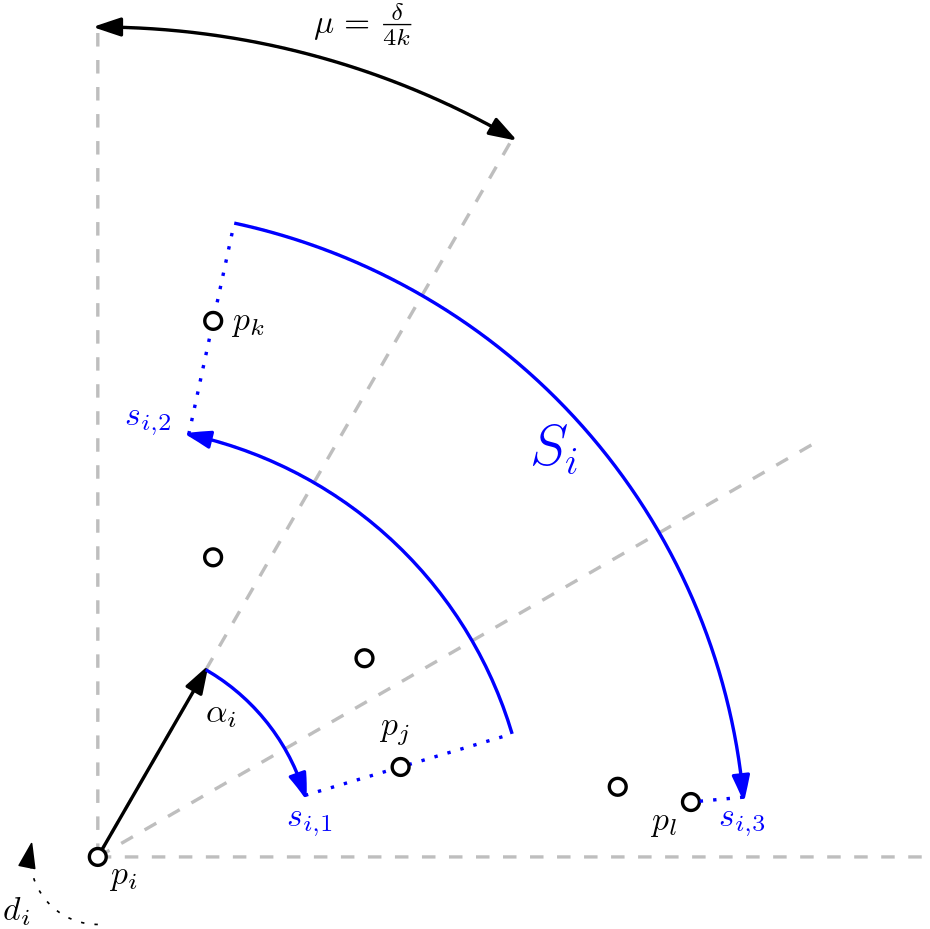
\includegraphics[height=7cm]{AFTP/algo1.png}}
    \only<2>{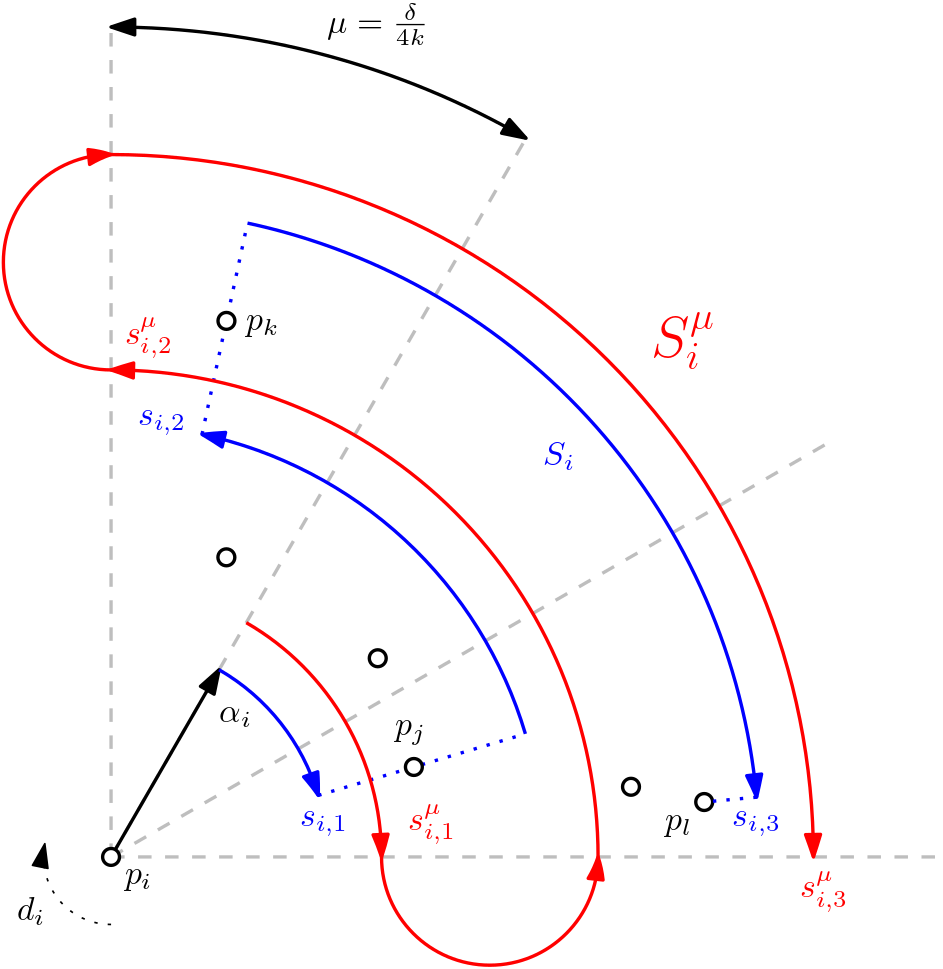
\includegraphics[height=7cm]{AFTP/algo2.png}}
  \end{minipage}
\end{frame}

\begin{frame}{Usando o Lema}
    Consideramos apenas soluções $\mu$-discretas cuja energia total não excede $(1 + \nicefrac{1}{k}) \cdot E$!
\end{frame}

\begin{frame}{Conclusão}
  \begin{itemize}[<+->]
    \item Após cada rotação, a antena de um satélite estará em uma das $O\left( \nicefrac{E}{\mu} \right)$ \textbf{orientações possíveis};

    \item Existem $O\left( \nicefrac{E^2}{\mu^2} \right)$ \textbf{transições válidas} por satélite, totalizando $O\left( n \cdot \nicefrac{E^2}{\mu^2} \right)$ transições;

    \item Apenas $O\left( \nicefrac{E}{\mu} \right)$ delas podem ser selecionadas;

    \bigbreak
    \item Total de $\binom{O\left( n \cdot \nicefrac{E^2}{\mu^2} \right)}{O\left( \nicefrac{E}{\mu} \right)}$ \textbf{soluções possíveis}, que podem ser checadas em tempo $\left( n \frac{E k}{\delta} \right)^{O\left( \nicefrac{E k}{\delta} \right)}$.
  \end{itemize}
\end{frame}
